\documentclass[10pt,pdf,intlimits]{beamer}
\usepackage[utf8]{inputenc}
\usepackage[russian]{babel}
\usefonttheme{professionalfonts}
\usepackage{beamerthemesplit}
\usetheme[numbers, totalnumbers, minimal, nonav, nologo]{Statmod}
\setbeamertemplate{caption}[numbered]
\setbeamertemplate{blocks}[rounded]
\setbeamertemplate{title page}[default][colsep=-4bp,rounded=true]
\setbeamertemplate{frametitle}[default][colsep=-4bp,rounded=true]
\setbeamercolor{normal text}{fg=black}
\setbeamercolor*{structure}{fg=black,bg=white}
\setbeamercolor*{palette primary}{use=structure,fg=black,bg=structure.bg}
\setbeamercolor*{palette secondary}{use=structure,fg=black,bg=structure.bg}
\setbeamercolor*{palette tertiary}{use=structure,fg=black,bg=structure.bg}
\setbeamerfont{footline}{series=\sffamily\fontseries{m}\fontsize{5}{6}\selectfont}
\setbeamersize{text margin left=5mm, text margin right=5mm}

\newcommand{\pder}[2] {\frac{\partial #1}{\partial #2}}
\newcommand{\ppder}[2]{\frac{\partial^2 #1}{\partial {#2}^2}}
\newcommand{\pcder}[3]{\frac{\partial^2 #1}{\partial #2 \partial #3}}
\newcommand{\der}[2]  {\frac{d #1}{d #2}}
\newcommand{\dder}[2] {\frac{d^2 #1}{d {#2}^2}}

\newcommand{\const}{\mathrm{const}}
\newcommand{\average}[1]{\left\langle #1 \right\rangle}
\newcommand{\abs}[1]{\left| #1 \right|}
\newcommand{\ds}{\displaystyle}
\newcommand{\D}{\Delta}
\newcommand{\dotunder}[1]{\d{#1}}
\renewcommand{\d}{\delta}
\newcommand{\eps}{\varepsilon}
\renewcommand{\phi}{\varphi}

\newcommand{\divergence}{\mathrm{div\,}}
\newcommand{\gradient}  {\mathrm{grad\,}}
\newcommand{\rotor}     {\mathrm{rot\,}}

\date{Волгоград, 2016}
\title{Влияние постоянного электрического поля на эффект двухволнового смешивания в графеновой сверхрешётке}
\author{Абдрахманов В. Л., гр. Ф-2н}
\institute{Руководитель --- д.ф.-м.н. Завьялов Д. В.}

\begin{document}
  \frame{\titlepage}
  \begin{frame}
  \frametitle{Цель и задачи}
  Цель работы: исследование влияния постоянного электрического поля на явления взаимного выпрямления в одномерной ГСР под воздействием двух линейно поляризованных волн с кратными частотами и общей плоскостью поляризации.

  \vspace*{4ex}
  Для достижения цели поставлены следующие задачи:
  \begin{itemize}
    \item получить зависимость тока продольного двухволнового выпрямления от поперечного постоянного электрического поля;
    \item получить зависимость тока поперечного двухволнового выпрямления от продольного постоянного электрического поля;
    \item изучить характер изменения вида зависимостей при изменении частоты высокочастотного поля.
  \end{itemize}
  \end{frame}
  \begin{frame}
    \frametitle{Графеновая сверхрешётка}
      \begin{figure}[h]
          \center
          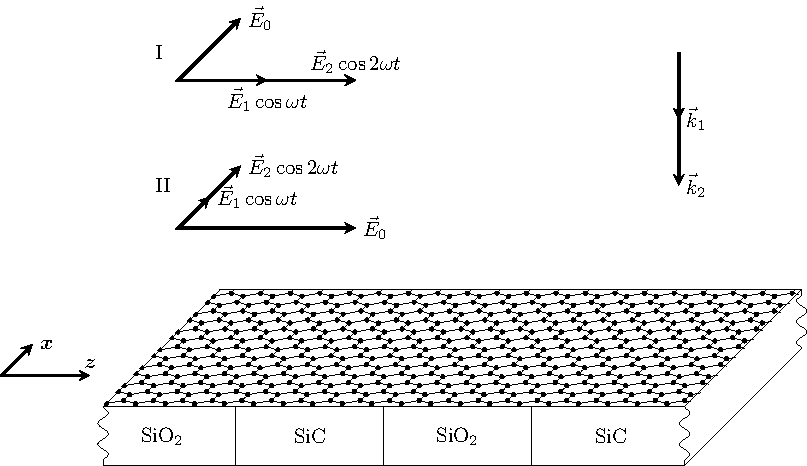
\includegraphics[height=.5\textheight]{../figures/graphene.pdf}
      \end{figure}
    \begin{equation}
      \eps(\vec{p}) = \sqrt{\Delta_g^2 + v_F^2 p_x^2} + \frac{\Delta_g}{\sqrt{\Delta_g^2 + v_F^2 p_x^2}}\Delta\left(1-\cos\frac{p_z d}{\hbar}\right),
    \end{equation}
    где \( \Delta_g = 0,\!059~\text{эВ} \), \( \Delta = 0,\!015~\text{эВ} \), \( d = 2 \cdot 10^{-6}~\text{см} \), \( v_F = 10^8~\frac{\text{см}}{\text{с}} \).
  \end{frame}
  \begin{frame}
  \frametitle{Квазиклассическое приближение}
  \begin{equation}
    \hbar\omega \ll \Delta_g,\quad eEd \ll \hbar\omega,\quad kT \ll \Delta_g      
  \end{equation}
  \begin{equation*}
      \omega \le 10^{13}~\text{рад}/\text{с},\quad E \le 10~\text{ед. СГС},\quad T\le100~\text{К}.
  \end{equation*}
  \begin{equation}
        \langle \vec{j} \rangle = \left\langle \int d^2 p  f(\vec{p}, t) \pder{\eps}{\vec{p}} \right\rangle
  \end{equation}
  Функцию распределения рассмотрим в приближении постоянного времени релаксации
  \begin{equation}
    f(t) = \frac{1}{\tau}\int_{-\infty}^{t} dt' \exp\left(\frac{t'-t}{\tau}\right) f_0(\vec{p'}),
  \end{equation}
  где
  \begin{equation}
    f_0 = C\exp\left[-\frac{\eps(\vec{p})}{kT}\right]
  \end{equation}
  есть равновесная функция распределения, а \( \vec{p'} \) удовлетворяет уравнению
  \begin{equation}
    \der{\vec{p'}}{t'} = e\vec{E},\quad \vec{p'}(t) = \vec{p}.
  \end{equation}
  \end{frame}
  \begin{frame}
  \frametitle{Влияние поперечного постоянного поля на продольное выпрямление}
        \begin{figure}[h]
          \center
          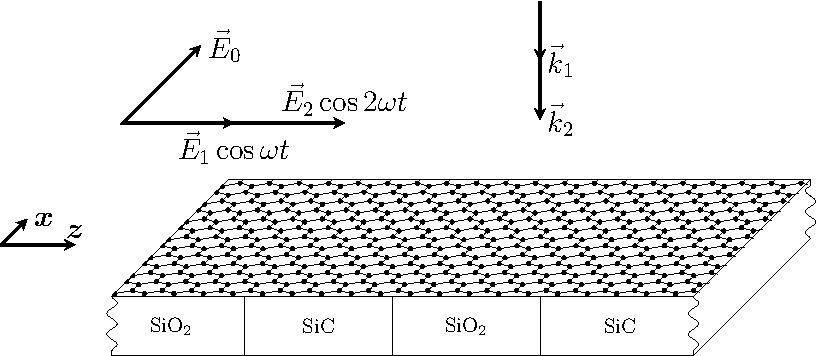
\includegraphics[height=.6\textheight]{../figures/graphene1.pdf}
      \end{figure}
  \end{frame}
  \begin{frame}
  \frametitle{Влияние поперечного постоянного поля на продольное выпрямление}
      \begin{align}
    \langle j_z \rangle &= 8\pi \frac{C\Delta_g\Delta}{v_F}\sum_{m=1}^\infty
    S_m\left(\frac{eE_1d}{\hbar\omega},\frac{eE_2d}{2\hbar\omega}\right)\times\\&\times
    \int_{-\infty}^\infty d\xi \exp\left[-\beta\left(\sqrt{1+\xi^2} +
    \frac{\Delta/\Delta_g}{\sqrt{1+\xi^2}}\right)\right]
    I_1\left(\frac{\Delta / kT}{\sqrt{1+\xi^2}}\right) R_m(\xi, \omega_0\tau,
    \omega\tau), \nonumber
\end{align}
\begin{equation}
      \omega_0 = \frac{e v_F}{\Delta_g}E_0,
\end{equation}
\begin{equation}
        R_m(a,b,c) = \int_0^\infty \frac{e^{-x}\sin
    (mcx)}{\sqrt{1+\left(a+bx\right)^2}}\,dx,
\end{equation}
\begin{equation}
    S_m(z_1,z_2) = \sum_{n=1}^\infty\sum_{k=-\infty}^\infty
   J_{m-2k+2n}(z_1)J_{m-2k-2n+2}(z_1)J_{k-n}(z_2)J_{k+n-1}(z_2).
\end{equation}
  \end{frame}
  \begin{frame}
    \frametitle{Влияние поперечного постоянного поля на продольное выпрямление}
        \begin{figure}[h]
          \center
          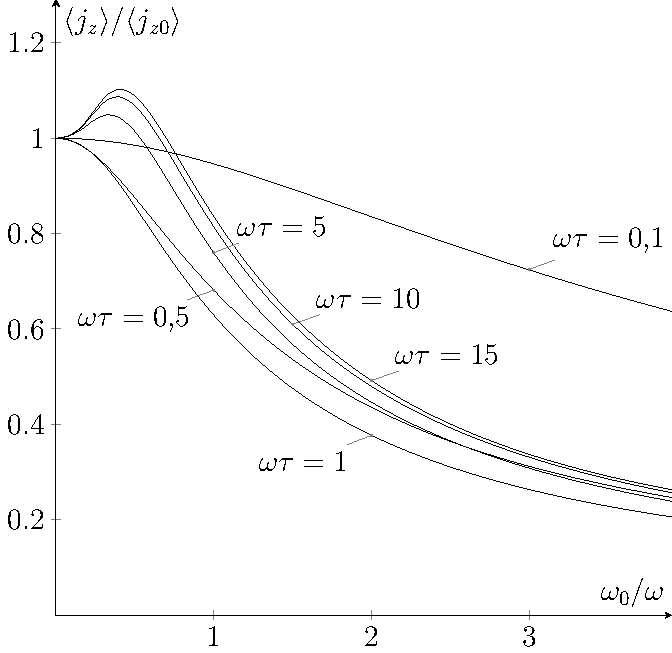
\includegraphics[height=.8\textheight]{../figures/jz.pdf}
      \end{figure}
  \end{frame}
    \begin{frame}
    \frametitle{Влияние продольного постоянного поля на поперечное выпрямление}
        \begin{figure}[h]
          \center
          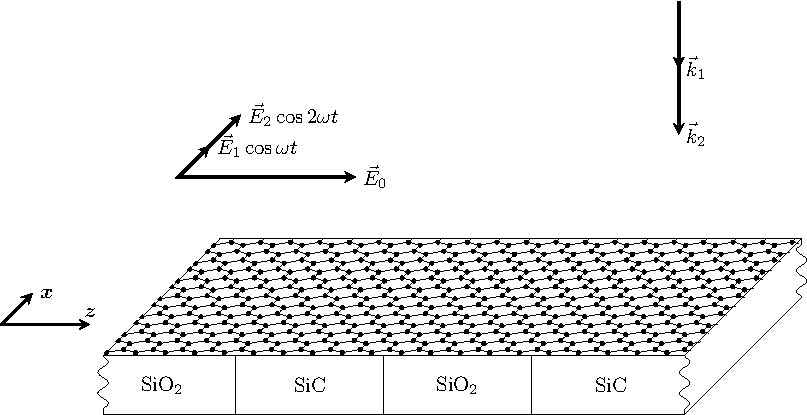
\includegraphics[height=.6\textheight]{../figures/graphene2.pdf}
      \end{figure}
  \end{frame}
  \begin{frame}
    \frametitle{Влияние продольного постоянного поля на поперечное выпрямление}
\begin{gather}
    \langle j_x \rangle = 2\omega\tau
    \frac{v_F^3}{\Delta_g^3}\frac{e^3}{\omega^3}E_1^2 E_2
    \cdot\Bigg[
        C_0\left(
            \frac{1}{1+4\omega^2\tau^2} -
            \frac{1}{1+\omega^2\tau^2}
            \right) + \nonumber \\+
        C_1\Bigg(
            \frac{1+(4\omega^2-\omega_0^2)\tau^2}
            {[1+(2\omega+\omega_0)^2\tau^2][1+(2\omega-\omega_0)^2\tau^2]}-\\-
            \frac{1+(\omega^2-\omega_0^2)\tau^2}
            {[1+(\omega+\omega_0)^2\tau^2][1+(\omega-\omega_0)^2\tau^2]}
            \Bigg)
    \Bigg], \nonumber
\end{gather}
\begin{equation}
  \omega_0 = \frac{ed}{\hbar}E_0.
\end{equation}
  \end{frame}
  \begin{frame}
    \frametitle{Влияние продольного постоянного поля на поперечное выпрямление}
        \begin{figure}[h]
          \center
          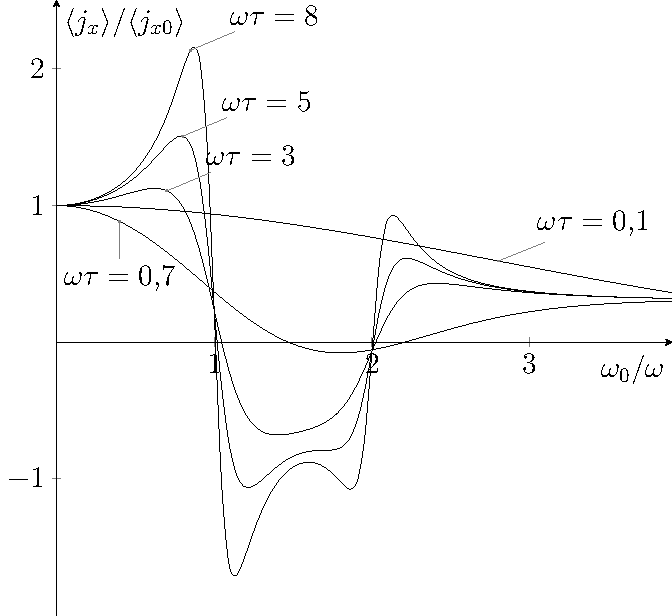
\includegraphics[height=.8\textheight]{../figures/jx.pdf}
      \end{figure}
  \end{frame}
  \begin{frame}
      \frametitle{Условия экспериментального наблюдения эффекта}
      \begin{equation}
          T = 77,\!4~\text{K},
      \end{equation}
      \begin{equation}
          \tau \sim 10^{-12}~\text{с},
      \end{equation}
      \begin{equation}
          n = 10^{10}~\text{см}^{-2},
      \end{equation}
      \begin{equation}
          E_1 = E_2 = 10~\text{ед. СГС},
      \end{equation}
      \begin{equation}
          \omega = 10^{12}~\text{рад}/\text{с},
      \end{equation}
      \begin{equation}
         \langle j_z \rangle \approx 10^{-6}~\text{А}/\text{см},
      \end{equation}
      \begin{equation}
          \langle j_x \rangle \approx 10^{-4}~\text{А}/\text{см}.
      \end{equation}
  \end{frame}
  \begin{frame}
      \frametitle{Заключение}
      \begin{enumerate}
        \item При продольном двухволновом выпрямлении приложенное поперечное постоянное электрическое поле приводит к уменьшению величины тока при малых частотах ВЧ поля (\(\omega\tau < 1\)). При  больших частотах (\(\omega\tau > 1\)) наблюдается увеличение тока в слабом поле, сменяющееся уменьшением в сильных полях. Резонансных явлений, подобных наблюдаемым в двухмерной СР, не обнаружено.
        \item При поперечном двухволновом выпрямлении приложенное продольное постоянное электрическое поле при малых частотах ВЧ поля (\(\omega\tau < 1\)) также приводит к уменьшению величины тока. Однако, при больших частотах (\(\omega\tau > 1\)) наблюдается резкое увеличение тока и смена его направления при приближении штарковской частоты к частоте одной из волн. Это связано с воздействием на блоховские осцилляции, вызванных постоянным электрическим полем, со стороны ВЧ поля.
        \item С ростом частоты падающих волн ток взаимного выпрямления убывает пропорционально 4 степени частоты, по крайней мере в одноминизонном приближении, когда энергия оптических квантов меньше ширины щели между минизонами.
    \end{enumerate}
  \end{frame}
\end{document}
